\clearpage
\refstepcounter{sourcechapter}
\phantomsection
\section*{附录 I\quad Curl 算子的性质及其对稳态 Navier--Stokes 方程的应用}
\label{app:curl-operator}
\addcontentsline{toc}{section}{附录 I\quad Curl 算子的性质及其对稳态 Navier--Stokes 方程的应用}
\setcounter{section}{0}
\MBSetSourceChapterAnchor{appendix-01}

\hypertarget{appendix-01-page-326}{}
本附录给出 $\mathbb R^n$, $n=2$ 或 $3$, 中有界集上 curl 算子的一些泛函性质, 并由这些性质导出第 2 章定理 \MBUnresolvedReference{theorem}{Theorem 1.5} 中存在性结果的一种改进形式. 我们主要遵循 C. Foias--R. Temam [3] 第 1 节.

\section{Curl 算子的泛函性质}
\label{sec:app1-functional-properties}

设 $\Omega$ 是 $\mathbb R^n$, $n=2$ 或 $3$, 中的有界开集. 假设:
\begin{equation}
\begin{minipage}{0.82\textwidth}
$\Omega$ 连通且为 $C^2$ 类(见第 1 章 \MBUnresolvedReference{equation}{(1.3)}), 其边界 $\Gamma$ 有有限个连通分支, 记为 $\Gamma_1,\ldots,\Gamma_k$ ($k\geq1$).
\end{minipage}
\label{eq:app1-domain-regularity}
\end{equation}
开集 $\Omega$ 可以单连通或多连通. 在后一种情形, 显然可用有限条光滑割面使之成为单连通集. 更确切地说:
\begin{equation}
\begin{minipage}{0.82\textwidth}
以 $\Sigma_1,\ldots,\Sigma_N$ 表示 $N$ 个 $n-1$ 维 $C^2$ 类流形($N\geq0$), 使 $i\neq j$ 时 $\Sigma_i\cap\Sigma_j=\varnothing$, 且开集
$\dot\Omega=\Omega\setminus\Sigma$, $\Sigma=\bigcup_{i=1}^N\Sigma_i$, 单连通并具有 Lipschitz 边界(即各 $\Sigma_i$ 不与 $\Gamma$ 相切).
\end{minipage}
\label{eq:app1-domain-cuts}
\end{equation}
其余记号与全书其他部分相同, 特别是第 1 章第 1, 2 节及第 2 章第 1 节引入的函数空间记号. 有时还要用到空间 $H^{m-1/2}(\Gamma)$, 其中整数 $m\geq1$; 它是 $\gamma_0H^m(\Omega)$, 即 $H^m(\Omega)$ 中函数的迹空间, 配备商范数
\begin{equation}
\lVert\psi\rVert_{H^{m-1/2}(\Gamma)}
=\inf_{\gamma_0u=\psi}\lVert u\rVert_{H^m(\Omega)}.
\label{eq:app1-trace-quotient-norm}
\end{equation}
这些空间的系统研究见 J.L. Lions--E. Magenes [1].

\begin{figure}[htbp]
\centering
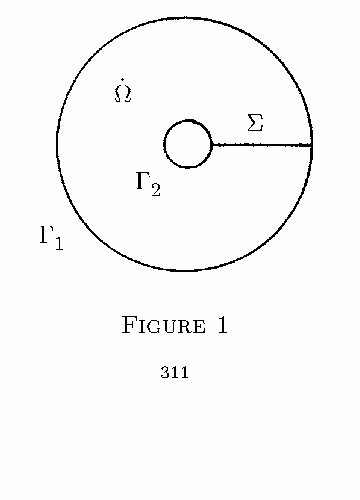
\includegraphics[width=0.28\textwidth]{figures/appendix01-figure01.png}
\caption{}
\label{fig:app1-domain-cut}
\end{figure}

\hypertarget{appendix-01-page-327}{}
还回顾第 1 章定理 \MBUnresolvedReference{theorem}{Theorem 1.5} 给出的 $L^2(\Omega)$ 正交分解
\begin{equation}
L^2(\Omega)=H\oplus H_1\oplus H_2,
\label{eq:app1-l2-orthogonal-decomposition}
\end{equation}
其中 $H_1,H_2$ 由第 1 章 \MBUnresolvedReference{equation}{(1.41)}, \MBUnresolvedReference{equation}{(1.42)} 定义. 下面将给出 $H$ 的一个正交分解.

\subsection{Curl 算子的核}
\label{subsec:app1-kernel-curl}

三维情形无需回顾 curl 算子的定义. 若 $n=2$, 约定
\[
\operatorname{curl}u=(-D_2u,D_1u),
\quad u:\Omega\to\mathbb R,
\]
\[
\operatorname{curl}u=D_1u_2-D_2u_1,
\quad u=\{u_1,u_2\}:\Omega\to\mathbb R^2.
\]
当 $n=3$ 时 curl 将 $L^2(\Omega)$ 映入 $H^{-1}(\Omega)$; 当 $n=2$ 时则映入 $H^{-1}(\Omega)$. 现在描述其在 $L^2$ 中的核 $\operatorname{Ker}(\operatorname{curl})$.

显然 $\operatorname{Ker}(\operatorname{curl})\supset H_1\oplus H_2$. 设 $u\in\operatorname{Ker}(\operatorname{curl})\cap H$. 则 $u$ 局部为梯度; 更确切地说, 在 $\dot\Omega$ 中 $u=\operatorname{grad}q$, 且 $\operatorname{div}u=\Delta q=0$. 因而 $q$ 在 $\dot\Omega$ 中单值且光滑, 除 $\Gamma\cap\Sigma$ 的邻域外在 $\overline{\dot\Omega}$ 中光滑. 由第 1 章 \MBUnresolvedReference{equation}{(1.34)}, 还有 $\partial q/\partial\nu=0$ 在 $\Gamma$ 上成立.

记 $\Sigma_i^+,\Sigma_i^-$ 为 $\Sigma_i$ 的两侧, $\nu_i$ 为从 $\Sigma_i^+$ 指向 $\Sigma_i^-$ 的单位法向量. 若函数 $\theta$ 在两侧取不同值, 令
\[
[\theta]_i=\theta|_{\Sigma_i^+}-\theta|_{\Sigma_i^-}.
\]
对上述 $q$, 因 $\operatorname{grad}q$ 单值且光滑, $[q]_i$ 是常数. 再由 $\operatorname{div}u=0$, 对任意 $\varphi\in\mathcal D(\Omega)$,
\[
\begin{aligned}
\langle\operatorname{div}u,\varphi\rangle
&=-\langle\operatorname{grad}q,\operatorname{grad}\varphi\rangle
=-\int_{\dot\Omega}\operatorname{grad}q\cdot\operatorname{grad}\varphi\,dx\\
&=-\int_{\partial\dot\Omega}\varphi\frac{\partial q}{\partial\nu}\,d\Gamma
=-\sum_{i=1}^N\int_{\Sigma_i}
\left[\frac{\partial q}{\partial\nu_i}\right]_i\varphi\,d\Sigma=0.
\end{aligned}
\]
故 $[\partial q/\partial\nu_i]_i=0$, $i=1,\ldots,N$.

\hypertarget{appendix-01-page-328}{}
\MBSourceStatementNumber{lemma}{1}
\begin{Lemma}
\label{lem:app1-kernel-characterization}
空间 $H_c=\operatorname{Ker}(\operatorname{curl})\cap H$ 由如下调和函数 $q$ 的梯度组成: $q$ 在 $\Omega$ 中多值, 在 $\dot\Omega$ 中单值, 并满足
\begin{equation}
\frac{\partial q}{\partial\nu}=0\quad\text{在 }\Gamma\text{ 上},
\label{eq:app1-kernel-boundary-normal}
\end{equation}
\begin{equation}
[q]_i=\text{常数},
\qquad i=1,\ldots,N,
\label{eq:app1-kernel-jumps}
\end{equation}
\begin{equation}
\left[\frac{\partial q}{\partial\nu_i}\right]_i=0,
\qquad i=1,\ldots,N.
\label{eq:app1-kernel-normal-jumps}
\end{equation}
\end{Lemma}

下面构造 $H_c$ 的一组基.

\MBSourceStatementNumber{lemma}{2}
\begin{Lemma}
\label{lem:app1-cut-potential-basis}
对 $i=1,\ldots,N$, 存在函数 $q_i$, 在相差一个加法常数的意义下唯一, 使
\begin{equation}
\left\{
\begin{aligned}
&\Delta q_i=0\quad\text{在 }\dot\Omega\text{ 中},
&&\frac{\partial q_i}{\partial\nu}=0\quad\text{在 }\Gamma\text{ 上},\\
&\left[\frac{\partial q_i}{\partial\nu_j}\right]_j=0,
&&j=1,\ldots,N,\\
&[q_i]_j=0,
&&j\neq i,\\
&[q_i]_i=1.
\end{aligned}
\right.
\label{eq:app1-normalized-cut-potential}
\end{equation}
\end{Lemma}

\begin{Proof}
考虑下述将证明与 \eqref{eq:app1-normalized-cut-potential} 等价的问题:
\begin{equation}
\left\{
\begin{aligned}
&\Delta q_i'=0\quad\text{在 }\dot\Omega\text{ 中},
&&\frac{\partial q_i'}{\partial\nu}=0\quad\text{在 }\Gamma\text{ 上},\\
&\left[\frac{\partial q_i'}{\partial\nu_j}\right]_j=0,
&&j=1,\ldots,N,\\
&[q_i']_j=0,
&&j\neq i,\\
&[q_i']_i=\text{未定常数},
&&\int_{\Sigma_i}\frac{\partial q_i'}{\partial\nu_i}\,d\Sigma=1.
\end{aligned}
\right.
\label{eq:app1-flux-normalized-cut-potential}
\end{equation}
这是一个变分问题. 令
\[
X_i=\{p\in H^1(\dot\Omega):[p]_i=\text{常数},
\ [p]_j=0, j\neq i\}.
\]
容易验证 \eqref{eq:app1-flux-normalized-cut-potential} 等价于求 $q_i'\in X_i$, 使
\begin{equation}
\int_\Omega\operatorname{grad}q_i'\cdot\operatorname{grad}p\,dx
=[p]_i,
\qquad\forall p\in X_i.
\label{eq:app1-cut-variational-problem}
\end{equation}
左端在 $X_i/\mathbb R$ 上定义连续强制双线性形式; 右端在常数上为零, 从而在 $X_i/\mathbb R$ 上诱导连续线性形式. 由第 1 章定理 \MBUnresolvedReference{theorem}{Theorem 2.2}, 得 $q_i'\in X_i/\mathbb R$ 的存在唯一性.

若 $q_i'$ 是 \eqref{eq:app1-cut-variational-problem} 的解, 则 $\alpha_i=[q_i']_i\neq0$, 且 $q_i=(1/\alpha_i)q_i'$ 是 \eqref{eq:app1-normalized-cut-potential} 的解. 否则 $q_i'$ 可延拓为 $H^1(\Omega)$ 中齐次 Neumann 问题的解, 因而为常数, 这与 \eqref{eq:app1-cut-variational-problem} 矛盾.

\hypertarget{appendix-01-page-329}{}
反之, 若 $q_i$ 是 \eqref{eq:app1-normalized-cut-potential} 的解, 则
\[
\beta_i=\int_{\Sigma_i}\frac{\partial q_i}{\partial\nu_i}\,d\Sigma\neq0,
\]
且 $q_i'=(1/\beta_i)q_i$ 是 \eqref{eq:app1-flux-normalized-cut-potential} 的解. 若 $\beta_i=0$, 则 $q_i$ 将是左端改为零的 \eqref{eq:app1-cut-variational-problem} 的解, 从而在 $X_i/\mathbb R$ 中为零, 与 $[q_i]_i=1$ 矛盾.
\end{Proof}

\MBSourceStatementNumber{lemma}{3}
\begin{Lemma}
\label{lem:app1-kernel-basis}
$H_c=\operatorname{Ker}(\operatorname{curl})\cap H$ 是由 $\operatorname{grad}q_1,\ldots,\operatorname{grad}q_N$ 张成的空间.\footnote{$\operatorname{grad}q_i$ 在这里按经典意义理解. $q_i$ 的分布梯度是这些函数与位于 $\Sigma_i$ 上的 Dirac 分布 $-[q_i]_i\nu_i\delta_{\Sigma_i}$ 之和.} 它的维数为 $N$.
\end{Lemma}

\begin{Proof}
若 $u\in H_c$, 则 $u=\operatorname{grad}q$, 其中 $q$ 满足引理 \ref{lem:app1-kernel-characterization} 的条件. 令 $a_i=[q]_i$, $r=q-\sum_{i=1}^Na_iq_i$. 显然 $r$ 在 $\dot\Omega$ 中解析, 且
\[
\Delta r=0\text{ 在 }\dot\Omega\text{ 中},
\quad\frac{\partial r}{\partial\nu}=0\text{ 在 }\Gamma\text{ 上},
\quad\left[\frac{\partial r}{\partial\nu_i}\right]_i=0,
\quad[r]_i=0.
\]
故 $r$ 是常数, $u=\sum_{i=1}^Na_i\operatorname{grad}q_i$. 函数 $\operatorname{grad}q_i$ 显然线性无关.
\end{Proof}

\MBSourceStatementNumber{remark}{1}
\begin{Remark}
\label{rem:app1-kernel-topology}
(i) 若 $\Omega$ 单连通, 则 $N=0$, $H_c=\{0\}$.

(ii) 空间 $H_c$ 同构于 $\Omega$ 的第一上同调空间, 即 $\Omega$ 上闭微分形式空间关于恰当微分形式空间的商(见 G. de Rham [1]).
\end{Remark}

\MBSourceStatementNumber{lemma}{4}
\begin{Lemma}
\label{lem:app1-H0-characterization}
设 $H_0$ 是 $H_c$ 在 $H$ 中的正交补. 则
\begin{equation}
H_0=\left\{v\in H:\int_{\Sigma_i}v\cdot\nu\,d\Sigma=0,
\ i=1,\ldots,N\right\}.
\label{eq:app1-H0-flux-characterization}
\end{equation}
\end{Lemma}

\begin{Proof}
若 $v\in H$, 则 $v\in H_0$ 当且仅当 $(v,\operatorname{grad}q_i)=0$, $i=1,\ldots,N$. 由第 1 章广义 Stokes 公式 \MBUnresolvedReference{equation}{(1.19)},
\[
(v,\operatorname{grad}q_i)
=\int_{\dot\Omega}v\cdot\operatorname{grad}q_i\,dx
=\int_{\partial\dot\Omega}v\cdot\nu q_i\,d\Gamma
=\int_{\Sigma_i}v\cdot\nu\,d\Sigma.
\]
于是得到 \eqref{eq:app1-H0-flux-characterization}.
\end{Proof}

\MBSourceStatementNumber{remark}{2}
\begin{Remark}
\label{rem:app1-cut-independence}
(i) 对 $v\in H$, $\int_{\Sigma_i}v\cdot\nu\,d\Sigma$ 与割面 $\Sigma_i$ 无关, 即其值在 $\Sigma_i$ 连续变形时不变.

(ii) 可直接验证: 若 $v\in H_c$, $v=\operatorname{grad}q$, 且 $\int_{\Sigma_i}v\cdot\nu\,d\Sigma=0$, $i=1,\ldots,N$, 则 $v=0$.
\end{Remark}

\hypertarget{appendix-01-page-330}{}
\begin{figure}[htbp]
\centering
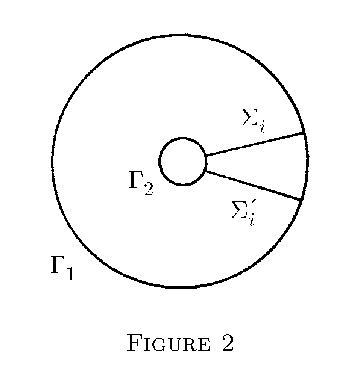
\includegraphics[width=0.28\textwidth]{figures/appendix01-figure02.png}
\caption{}
\label{fig:app1-deformed-cut}
\end{figure}

\MBSourceStatementNumber{proposition}{1}
\begin{Proposition}
\label{prop:app1-orthogonal-decomposition}
在假设 \eqref{eq:app1-domain-regularity}, \eqref{eq:app1-domain-cuts} 下,
\begin{equation}
L^2(\Omega)=H_c\oplus H_0\oplus H_1\oplus H_2,
\label{eq:app1-full-l2-decomposition}
\end{equation}
\begin{equation}
\operatorname{Ker}(\operatorname{curl})=H_c\oplus H_1\oplus H_2,
\label{eq:app1-full-kernel-decomposition}
\end{equation}
其中 $H_c,H_0,H_1,H_2$ 如上所述.
\end{Proposition}

\MBSourceStatementNumber{remark}{3}
\begin{Remark}
\label{rem:app1-projectors}
(i) 记 $P_{H_c},P_{H_i}$ 为 $L^2(\Omega)$ 到 $H_c,H_i$, $i=0,1,2$, 上的正交投影. $P_{H_1},P_{H_2}$ 已在第 1 章定理 \MBUnresolvedReference{theorem}{Theorem 1.5} 的证明和注 \MBUnresolvedReference{remark}{Remark 1.6} 中隐式引入并定义. 若 $u\in L^2(\Omega)$,
\begin{equation}
u_2=P_{H_2}u=\operatorname{grad}p,
\label{eq:app1-H2-projection}
\end{equation}
其中 $p$ 是 Dirichlet 问题
\begin{equation}
\Delta p=\operatorname{div}u\in H^{-1}(\Omega),
\qquad p\in H_0^1(\Omega)
\label{eq:app1-H2-dirichlet-problem}
\end{equation}
的解, 且
\begin{equation}
u_1=P_{H_1}u=\operatorname{grad}q,
\label{eq:app1-H1-projection}
\end{equation}
其中 $q$ 是 Neumann 问题
\begin{equation}
\Delta q=0\quad\text{在 }\Omega\text{ 中},
\qquad\frac{\partial q}{\partial\nu}=\gamma_\nu(u-\operatorname{grad}p)
\quad\text{在 }\Gamma\text{ 上}
\label{eq:app1-H1-neumann-problem}
\end{equation}
的解. 该问题适定(见第 1 章 \MBUnresolvedReference{equation}{(1.44)} 及其后的注释).

$P_{H_c}$ 定义如下: $P_{H_c}u=\sum_{i=1}^Na_i\operatorname{grad}q_i$, 其中 $a_i$ 是线性系统
\begin{equation}
\sum_{i=1}^N\alpha_{ij}a_i
=\int_{\Sigma_j}u\cdot\nu\,d\Sigma,
\qquad1\leq j\leq N,
\label{eq:app1-Hc-projection-system}
\end{equation}
的解, 且
\[
\alpha_{ij}=\int_{\Sigma_j}\frac{\partial q_i}{\partial\nu_j}\,d\Sigma
=\int_{\Sigma_i}\frac{\partial q_j}{\partial\nu_i}\,d\Sigma
=(\operatorname{grad}q_i,\operatorname{grad}q_j).
\]
因此矩阵 $(\alpha_{ij})$ 可逆.

(ii) 已知若 $\Omega$ 为 $C^r$ 类, $r\geq m+2$, 则 $P_{H_1},P_{H_2}$ 将 $H^m(\Omega)$ 映入 $H_i\cap H^m(\Omega)$. 因为 $H_c\subset C^\infty(\Omega)\cap C^r(\overline\Omega)$, $P_{H_c},P_{H_0}$ 也有相同性质.
\end{Remark}

\hypertarget{appendix-01-page-331}{}
\subsection{空间 $\operatorname{curl}(H^1(\Omega))$}
\label{subsec:app1-curl-H1}

\MBSourceStatementNumber{lemma}{5}
\begin{Lemma}
\label{lem:app1-curl-H1-H0}
\[
\operatorname{curl}H^1(\Omega)
=\operatorname{curl}(H^1(\Omega)\cap H_0).
\]
\end{Lemma}

\begin{Proof}
若 $u\in H^1(\Omega)$, 令 $v=P_{H_0}u=u-\operatorname{grad}q$, 其中 $\operatorname{grad}q\in\operatorname{Ker}(\operatorname{curl})$, 因而 $\operatorname{curl}v=\operatorname{curl}u$.
\end{Proof}

\MBSourceStatementNumber{lemma}{6}
\begin{Lemma}
\label{lem:app1-curl-poincare}
存在常数 $c_0=c_0(\Omega)$, 使对每个 $u\in H^1(\Omega)\cap H_0$,
\begin{equation}
\lVert u\rVert_{H^1(\Omega)}\leq c_0|\operatorname{curl}u|,
\label{eq:app1-curl-H1-estimate}
\end{equation}
\begin{equation}
|u|\leq c_0|\operatorname{curl}u|.
\label{eq:app1-curl-L2-estimate}
\end{equation}
\end{Lemma}

\begin{Proof}
G. Duvaut--J.L. Lions [1] (第 7 章定理 6.1)证明
\begin{equation}
\{u\in H^1(\Omega):\gamma_\nu u=u\cdot\nu|_\Gamma=0\}
=\{u\in L^2(\Omega):\operatorname{div}u,\operatorname{curl}u\in L^2(\Omega),
\ \gamma_\nu u=0\text{ 在 }\Gamma\text{ 上}\},
\label{eq:app1-div-curl-trace-space}
\end{equation}
且存在 $c_1=c_1(\Omega)$, 使此空间中每个 $u$ 满足
\begin{equation}
\lVert u\rVert_{H^1(\Omega)}
\leq c_1\{|u|+|\operatorname{div}u|+|\operatorname{curl}u|\}.
\label{eq:app1-div-curl-H1-estimate}
\end{equation}
因此 \eqref{eq:app1-curl-H1-estimate} 是 \eqref{eq:app1-curl-L2-estimate}, \eqref{eq:app1-div-curl-H1-estimate} 的直接推论.

用反证法证明 \eqref{eq:app1-curl-L2-estimate}. 若它不成立, 则存在序列 $u_m\in H^1(\Omega)\cap H_0$, 使
\begin{equation}
|u_m|>m|\operatorname{curl}u_m|,
\qquad\forall m.
\label{eq:app1-curl-contradiction-sequence}
\end{equation}
可设 $|u_m|=1$. 由 \eqref{eq:app1-div-curl-H1-estimate}, $u_m$ 在 $H^1(\Omega)$ 中有界. 可抽取仍记作 $u_m$ 的子列, 它在 $H^1(\Omega)$ 中弱收敛到 $u\in H^1(\Omega)\cap H_0$, 在 $L^2(\Omega)$ 中强收敛, 因而 $|u|=1$. 另一方面, 由 \eqref{eq:app1-curl-contradiction-sequence}, $u\in H_0\cap\operatorname{Ker}(\operatorname{curl})$, 故 $u=0$, 矛盾.
\end{Proof}

\MBSourceStatementNumber{lemma}{7}
\begin{Lemma}
\label{lem:app1-curl-range-closed}
当 $n=3$ 时, $\operatorname{curl}H^1(\Omega)$ 在 $L^2(\Omega)$ 中闭; 当 $n=2$ 时, 它在 $L^2(\Omega)$ 中闭.
\end{Lemma}

\begin{Proof}
由 \eqref{eq:app1-curl-H1-estimate}, curl 是从 $H^1(\Omega)\cap H_0$ 到 $L^2(\Omega)$ (二维时到 $L^2(\Omega)$)的同构.
\end{Proof}

\paragraph{$(\operatorname{curl}H^1(\Omega))^\perp$ 的刻画.}

\MBSourceStatementNumber{proposition}{2}
\begin{Proposition}
\label{prop:app1-curl-orthogonal-complement}
若 $n=3$, 则
\[
(\operatorname{curl}H^1(\Omega))^\perp
=\{u\in L^2(\Omega):u=\operatorname{grad}p,
\ p\in H^1(\Omega),\ p\text{ 在每个 }\Gamma_i\text{ 上为常数}\}.
\]
\end{Proposition}

\begin{Proof}
若 $u\in(\operatorname{curl}H^1(\Omega))^\perp$, 则
\[
(u,\operatorname{curl}\varphi)=0,
\qquad\forall\varphi\in\mathcal D(\Omega),
\]
故 $\operatorname{curl}u=0$. 因 $u,\operatorname{curl}u\in L^2(\Omega)$, 由 G. Duvaut--J.L. Lions [1] 的迹定理可定义 $u\wedge\nu|_\Gamma\in H^{-1/2}(\Gamma)$, 并有广义 Stokes 公式
\begin{equation}
(u,\operatorname{curl}\varphi)
=(\operatorname{curl}u,\varphi)
+\langle u\wedge\nu|_\Gamma,\gamma_0\varphi\rangle,
\qquad\forall\varphi\in H^1(\Omega).
\label{eq:app1-generalized-curl-stokes}
\end{equation}

\hypertarget{appendix-01-page-332}{}
于是 $u\wedge\nu|_\Gamma=0$, 且
\[
(\operatorname{curl}H^1(\Omega))^\perp
=\{u\in L^2(\Omega):\operatorname{curl}u=0,
\ u\wedge\nu|_\Gamma=0\}.
\]
更精确地, 这样的 $u$ 满足 $u=\operatorname{grad}p$, 且 $u\in H_c\oplus H_1\oplus H_2$. 因 $\operatorname{grad}p=(\partial p/\partial\nu)\nu+\nabla_\tau p$, 条件 $u\wedge\nu|_\Gamma=0$ 等价于 $\nabla_\tau p=0$ 在 $\Gamma$ 上成立, 即 $p$ 在每个 $\Gamma_i$ 上为常数. 必有 $P_{H_c}(\operatorname{grad}p)=0$, 因而 $p\in H^1(\Omega)$. 逆命题容易验证.
\end{Proof}

\MBSourceStatementNumber{proposition}{3}
\begin{Proposition}
\label{prop:app1-curl-range-characterization}
在假设 \eqref{eq:app1-domain-regularity}, \eqref{eq:app1-domain-cuts} 下, 若 $n=3$, 则
\[
\operatorname{curl}H^1(\Omega)
=\left\{u\in L^2(\Omega):\operatorname{div}u=0,
\ \int_{\Gamma_i}u\cdot\nu\,d\Gamma=0,
\ \forall i\right\}.
\]
\end{Proposition}

\begin{Proof}
记右端空间为 $Y$. 因 $\operatorname{curl}(H^1(\Omega))$ 闭, 只需证明 $Y=(\operatorname{curl}H^1(\Omega))^{\perp\perp}$. 若 $v=\operatorname{grad}p\in(\operatorname{curl}H^1(\Omega))^\perp$, $u\in L^2(\Omega)$ 且 $\operatorname{div}u=0$, 则
\[
(u,v)=\int_\Omega u\cdot\operatorname{grad}p\,dx
=\int_\Gamma\gamma_\nu u\,p\,d\Gamma
=\sum_{i=1}^kp(\Gamma_i)\int_{\Gamma_i}\gamma_\nu u\,d\Gamma.
\]
由于 $p(\Gamma_i)$ 可任意取值, 结论成立.
\end{Proof}

\MBSourceStatementNumber{remark}{4}
\begin{Remark}
\label{rem:app1-connected-boundary-curl-range}
若 $\Gamma$ 连通, $k=1$, 则只剩
\[
\operatorname{curl}H^1(\Omega)
=\{u\in L^2(\Omega):\operatorname{div}u=0\}.
\]
\end{Remark}

\MBSourceStatementNumber{remark}{5}
\begin{Remark}
\label{rem:app1-two-dimensional-analogue}
若 $n=2$, 对 $\operatorname{curl}H^1(\Omega)$ 及其正交补有证明相同的类似结果.
\end{Remark}

\subsection{关于正则性的注记}
\label{subsec:app1-regularity}

下面补充 G. Duvaut--J.L. Lions 在 \eqref{eq:app1-div-curl-trace-space}, \eqref{eq:app1-div-curl-H1-estimate} 中的结果.

\MBSourceStatementNumber{proposition}{4}
\begin{Proposition}
\label{prop:app1-div-curl-regularity}
设 $\Omega\subset\mathbb R^n$, $n=2,3$, 是有界开集, $m\geq1$ 为整数. 假设 \eqref{eq:app1-domain-regularity}, \eqref{eq:app1-domain-cuts} 成立, 且 $\Omega$ 为 $C^r$ 类, $r\geq m+1$. 则
\begin{equation}
\begin{aligned}
H^m(\Omega)=\{u\in L^2(\Omega):
&\operatorname{curl}u\in H^{m-1}(\Omega),
\ \operatorname{div}u\in H^{m-1}(\Omega),\\
&\gamma_\nu u\in H^{m-1/2}(\Gamma)\},
\end{aligned}
\label{eq:app1-div-curl-regularity-space}
\end{equation}
且存在 $c_2=c_2(m,\Omega)$, 使每个 $u\in H^m(\Omega)$ 满足
\begin{equation}
\lVert u\rVert_{H^m(\Omega)}
\leq c_2\{|u|+\lVert\operatorname{curl}u\rVert_{H^{m-1}(\Omega)}
+|\operatorname{div}u|_{H^{m-1}(\Omega)}
+|\gamma_\nu u|_{H^{m-1/2}(\Gamma)}\}.
\label{eq:app1-div-curl-regularity-estimate}
\end{equation}
\end{Proposition}

\hypertarget{appendix-01-page-333}{}
\begin{Proof}
(i) 先取 $m=1$. \eqref{eq:app1-div-curl-regularity-space} 右端空间包含 $H^1(\Omega)$, 需证另一包含关系. 设 $u$ 属于该空间, $\operatorname{grad}p$ 是 $u$ 到 $H_1\oplus H_2$ 上的投影. 已知 $p$ 是 Neumann 问题
\begin{equation}
\Delta p=\operatorname{div}u\quad\text{在 }\Omega\text{ 中},
\qquad\frac{\partial p}{\partial\nu}=u\cdot\nu
\quad\text{在 }\Gamma\text{ 上}
\label{eq:app1-neumann-regularity-problem}
\end{equation}
的解. 令 $v=u-\operatorname{grad}p$. 则 $v,\operatorname{curl}v,\operatorname{div}v\in L^2(\Omega)$ 且 $\gamma_\nu v=0$, 所以由 \eqref{eq:app1-div-curl-trace-space}, $v\in H^1(\Omega)$. 由 Neumann 问题的标准正则性结果, $p\in H^2(\Omega)$, 故 $u\in H^1(\Omega)$. \eqref{eq:app1-div-curl-regularity-estimate} 由 \eqref{eq:app1-div-curl-H1-estimate} 和
\[
\lVert p\rVert_{H^2(\Omega)/\mathbb R}
\leq c_3\left\{|\Delta p|_{L^2(\Omega)}
+\left|\frac{\partial p}{\partial\nu}\right|_{H^{1/2}(\Gamma)}\right\}
\]
推出(见 Agmon--Douglis--Nirenberg [1] 或 Lions--Magenes [1]).

(ii) 当 $m>1$ 时用归纳法. 假设阶数 $m-1$ 时结论成立. 若 $u$ 属于 \eqref{eq:app1-div-curl-regularity-space} 右端, 则由归纳假设 $u\in H^{m-1}(\Omega)$. 对任意 $m-1$ 阶微分算子 $D^{m-1}$, $v=D^{m-1}u$ 满足
\[
v,\operatorname{curl}v,\operatorname{div}v\in L^2(\Omega),
\]
\[
v\cdot\nu
=D^{m-1}(u\cdot\nu)
-\sum_{i=1}^{m-1}\binom{m-1}{i}D^i\nu\,D^{m-1-i}u
\in H^{1/2}(\Gamma).
\]
由第一部分 $v\in H^1(\Omega)$, 所以 $u\in H^m(\Omega)$, 且 \eqref{eq:app1-div-curl-regularity-estimate} 易得.
\end{Proof}

\MBSourceStatementNumber{remark}{6}
\begin{Remark}
\label{rem:app1-regularity-refinements}
(i) 也可直接由 Agmon--Douglis--Nirenberg [1] 推出命题 \ref{prop:app1-div-curl-regularity}.

(ii) 可将 \eqref{eq:app1-div-curl-regularity-estimate} 替换为
\begin{equation}
\begin{aligned}
\lVert u-P_{H_c}u\rVert_{H^m(\Omega)}
\leq c_3\{&\lVert\operatorname{curl}u\rVert_{H^{m-1}(\Omega)}
+|\operatorname{div}u|_{H^{m-1}(\Omega)}\\
&+|\gamma_\nu u|_{H^{m-1/2}(\Gamma)}\}.
\end{aligned}
\label{eq:app1-div-curl-projected-estimate}
\end{equation}
\end{Remark}

\section{对非齐次稳态 Navier--Stokes 方程的应用}
\label{sec:app1-nonhomogeneous-steady}

当 $n=2$ 或 $3$ 时, 下述结果补充第 2 章定理 \MBUnresolvedReference{theorem}{Theorem 1.5}.

\MBSourceStatementNumber{theorem}{1}
\begin{Theorem}
\label{thm:app1-nonhomogeneous-existence}
假设 $n=2$ 或 $3$, 且 \eqref{eq:app1-domain-regularity}, \eqref{eq:app1-domain-cuts} 成立. 给定 $f\in H^{-1}(\Omega)$ 和 $\varphi\in H^{1/2}(\Gamma)$, 满足
\begin{equation}
\int_{\Gamma_i}\varphi\cdot\nu\,d\Gamma=0,
\qquad i=1,\ldots,k.
\label{eq:app1-boundary-component-flux}
\end{equation}
则第 2 章问题 \MBUnresolvedReference{equation}{(1.62)}--\MBUnresolvedReference{equation}{(1.64)} 至少有一个解 $u\in H^1(\Omega)$, $p\in L^2(\Omega)$.
\end{Theorem}

\begin{Proof}
由第 2 章定理 \MBUnresolvedReference{theorem}{Theorem 1.5}, 只须证明 $\varphi$ 满足第 2 章条件 \MBUnresolvedReference{equation}{(1.65)}, \MBUnresolvedReference{equation}{(1.66)}, 即
\begin{equation}
\varphi\in\gamma_0\{\operatorname{curl}H^2(\Omega)\}.
\label{eq:app1-boundary-curl-trace}
\end{equation}

\hypertarget{appendix-01-page-334}{}
设 $\varphi$ 满足 \eqref{eq:app1-boundary-component-flux}. 解非齐次 Stokes 问题
\[
-\Delta\Phi+\operatorname{grad}\pi=0,
\quad\operatorname{div}\Phi=0\text{ 在 }\Omega\text{ 中},
\quad\Phi=\varphi\text{ 在 }\Gamma\text{ 上},
\]
由第 1 章定理 \MBUnresolvedReference{theorem}{Theorem 2.4}, 得 $\Phi\in H^1(\Omega)$, $\operatorname{div}\Phi=0$, $\varphi=\gamma_0\Phi$. 由 \eqref{eq:app1-boundary-component-flux}, 引理 \ref{lem:app1-curl-H1-H0} 和命题 \ref{prop:app1-curl-range-characterization}, 存在 $\zeta\in H^1(\Omega)\cap H_0$, 使 $\operatorname{curl}\zeta=\Phi$. 注意 $\operatorname{curl}\zeta\in H^1(\Omega)$, 使用命题 \ref{prop:app1-div-curl-regularity}, 得 $\zeta\in H^2(\Omega)$, 因而 \eqref{eq:app1-boundary-curl-trace} 成立.
\end{Proof}

\MBSourceStatementNumber{remark}{1}
\begin{Remark}
\label{rem:app1-total-flux-necessary}
与第 1 章 \MBUnresolvedReference{equation}{(2.49)} 相同, $\varphi$ 的必要条件为
\begin{equation}
\int_\Gamma\varphi\cdot\nu\,d\Gamma=0,
\label{eq:app1-total-boundary-flux}
\end{equation}
它弱于 \eqref{eq:app1-boundary-component-flux}.
\end{Remark}

\MBSourceStatementNumber{remark}{2}
\begin{Remark}
\label{rem:app1-solution-regularity-reference}
关于 $u,p$ 的正则性, 见第 2 章注 \MBUnresolvedReference{remark}{Remark 1.6} 和命题 \MBUnresolvedReference{proposition}{Proposition 1.1}.
\end{Remark}

\MBSourceStatementNumber{remark}{3}
\begin{Remark}
\label{rem:app1-leray-smooth-solutions}
对多次连续可微的给定 $f,\varphi$, 若 $\varphi$ 满足 \eqref{eq:app1-boundary-component-flux}, J. Leray 在 [1] 中证明了第 2 章 \MBUnresolvedReference{equation}{(1.62)}--\MBUnresolvedReference{equation}{(1.64)} 存在多次连续可微的解.
\end{Remark}

\MBSourceStatementNumber{proposition}{1}
\begin{Proposition}
\label{prop:app1-boundary-lifting}
在定理 \ref{thm:app1-nonhomogeneous-existence} 的假设下, 对任意 $\delta>0$, 存在从
\begin{equation}
\dot H^{3/2}(\Gamma)
=\left\{\varphi\in H^{3/2}(\Gamma):
\int_{\Gamma_i}\varphi\cdot\nu\,d\Gamma=0,
\ i=1,\ldots,k\right\}
\label{eq:app1-boundary-lifting-domain}
\end{equation}
到 $H^2(\Omega)$ 的连续线性映射 $\Lambda_\delta$, 使
\begin{equation}
\operatorname{div}\Lambda_\delta\varphi=0
\quad\text{在 }\Omega\text{ 中},
\label{eq:app1-boundary-lifting-divergence}
\end{equation}
\begin{equation}
\gamma_0\Lambda_\delta\varphi=\varphi
\quad\text{在 }\Gamma\text{ 上},
\label{eq:app1-boundary-lifting-trace}
\end{equation}
\begin{equation}
|b(v,\Lambda_\delta\varphi,v)|
\leq\delta\lVert\varphi\rVert_{H^{3/2}(\Gamma)}\lVert v\rVert^2,
\qquad\forall\varphi\in\dot H^{3/2}(\Gamma),
\quad\forall v\in V.
\label{eq:app1-boundary-lifting-trilinear}
\end{equation}
\end{Proposition}

\begin{Proof}
只须分析上述定理 \ref{thm:app1-nonhomogeneous-existence} 和第 2 章定理 \MBUnresolvedReference{theorem}{Theorem 1.5} 的证明. 在定理 \ref{thm:app1-nonhomogeneous-existence} 的证明中, 映射 $\varphi\mapsto\Phi$ 从 $\dot H^{3/2}(\Gamma)$ 到 $H^2(\Omega)$ 连续线性. 由命题 \ref{prop:app1-curl-range-characterization}, \ref{prop:app1-div-curl-regularity},
\[
\operatorname{curl}H^2(\Omega)
=\{u\in H^1(\Omega):\operatorname{div}u=0,
\ \int_{\Gamma_i}u\cdot\nu\,d\Gamma=0,
\ \forall i\},
\]
且 curl 是从 $H^2(\Omega)\cap H_0$ 到 $\operatorname{curl}H^2(\Omega)$ 的同构. 因而 $\Phi=\operatorname{curl}\zeta$, $\zeta\in H^2(\Omega)\cap H_0$, 映射 $\Phi\mapsto\zeta$ 连续线性.

再分析第 2 章定理 \MBUnresolvedReference{theorem}{Theorem 1.5} 的证明, 即对应 $\varphi=\operatorname{curl}\zeta\mapsto\psi=\operatorname{curl}(\theta_\epsilon\zeta)$. 映射 $\zeta\mapsto\theta_\epsilon\zeta$ 显然在 $H^2(\Omega)$ 中连续线性. 当 $\epsilon$ 足够小, $\epsilon\leq\epsilon_0(\delta)$ 时, 可取 $\Lambda_\delta\varphi=\psi=\operatorname{curl}(\theta_\epsilon\zeta)$; 于是 \eqref{eq:app1-boundary-lifting-trilinear} 成立, 而 \eqref{eq:app1-boundary-lifting-divergence}, \eqref{eq:app1-boundary-lifting-trace} 显然成立(关于 \eqref{eq:app1-boundary-lifting-trilinear}, 见第 2 章 \MBUnresolvedReference{equation}{(1.85)}).
\end{Proof}

\hypertarget{appendix-01-page-335}{}
\MBSourceStatementNumber{remark}{4}
\begin{Remark}
\label{rem:app1-evolution-nonhomogeneous-boundary}
利用命题 \ref{prop:app1-boundary-lifting}, 容易建立类似于第 3 章第 3, 4 节的存在唯一性结果, 但速度满足非齐次边界条件
\[
u(x,t)=\varphi(x,y),
\qquad x\in\Gamma,\quad 0<t<T.
\]
这留作练习.
\end{Remark}
